%\documentclass{article}
%\usepackage[utf8]{inputenc}
%\usepackage{graphicx}
%\usepackage{float}
\renewcommand*\descriptionlabel[1]{\hspace\leftmargin$#1$}


\section{Literature Review}

\subsection{Molten Salt Reactors}

Modeling and simulation of liquid fueled molten salt reactors (MSRs) is different from modeling and simulation of solid fueled reactors in a few different areas. Two main areas of particular importance are the online reprocessing functionality and the movement of the fuel through the reactor. The online reprocessing functionality involves removing fission products from the fuel and adding fresh fuel during operation. The movement of the fuel causes a shift in the location of delayed neutron precursors (DNPs). In solid fueled reactors, the distribution of DNPs follows the flux profile, while in MSRs the DNPs move along with the fuel. This results in a reduction in the effective delayed neutron fraction due to decay of DNPs in less important regions.

\subsubsection{Online Reprocessing}

The online reprocessing functionality of MSRs is simulated in different ways depending on the particular software used and the overall approach can vary. The two main ways to approach the online reprocessing problem is by either using batch-wise reprocessing or continuous reprocessing. There are also different approaches in terms of modeling the full core and using a unit-cell model. 

Batchwise reprocessing is implemented by running the simulation, stopping, and then adding and removing materials. The simulation is then restarted and the process iterates. This method is useful in that it is fairly straightforward to implement, can be calibrated to different removal efficiencies directly, and scales with accuracy based on time step size. Some issues with the batchwise approach are that using large time steps will make the results more inaccurate, it has increased computational cost with smaller time steps, and it is an approximation of the actual physical process of reprocessing.

Continuous reprocessing is implemented by adding terms to the Bateman equation similar to an extra decay term. The benefits of using continuous reprocessing are that the model is physically accurate, it doesn't impact computational cost as much as a batchwise process, and it allows for large time steps to be used. A note should be made, however, that the time step size is still limited since the simulation will need to update based on the new material composition and evolving neutron spectrum. However, there is less error from inaccurate material removal and addition. The main downside of the continuous removal approach is that it is more cumbersome to implement and configure due to the nature of how it operates.

Imagine a process exists in which $X$\% of some element is removed from the fuel salt in the system over some time period T. For a batchwise approach, a straightforward approach would be to run the system, deplete for some time step $\tau$, remove $\gamma$\%, and repeat. The scaling term $\gamma$ for the removal efficiency is a linear approximation of the removal efficiency based on the time step adjustment and can be seen in Equation \ref{eq:batchwise_rem_eff}. An alternative approach is to establish a depletion time step $\tau$ such that the efficiency based time value $T$ is a multiple of $\tau$ and only have the batchwise removal occur at the steps when $\tau$ is a multiple of $T$. 

\begin{equation} \hfill 
\gamma = X \frac{\tau}{T}
\hfill\label{eq:batchwise_rem_eff} \end{equation}

For a continuous approach, removing some fraction is dependent upon the particular isotope since the approach involves adding a term to the Bateman equation. This is one of the methods used in Serpent2 continuous reprocessing, where separations are only performed based on the element, not each particular isotope, an extension developed by Aufiero et al \cite{aufiero_extended_2013} \cite{auero_modication_nodate}. Equation \ref{eq:Bateman_default} shows the generic form of the Bateman equation, while Equation \ref{eq:Bateman_type_one_decay} shows the terms added to Equation \ref{eq:Bateman_default}, which are the reprocessing constants, or $\lambda_{r}$ added. 

\begin{equation} \hfill
%\frac{dN}{dt} = \sum_j \lambda_j N_j + \gamma \Sigma_f \phi + \Sigma_k \phi - \lambda N - \Sigma \phi - C
\frac{dN_j}{dt}_{base} = \sum_{i \neq j} \left [ \left( \gamma_{i \rightarrow j} \sigma_{f, i} \Phi + \lambda _{i \rightarrow j} + \sigma_{i \rightarrow j} \Phi \right) N_i \right ] - \left ( \lambda_j + \sigma_j \Phi \right ) N_j
\hfill\label{eq:Bateman_default} \end{equation}

\begin{equation} \hfill
%\frac{dN}{dt} = \sum_j \lambda_j N_j + \gamma \Sigma_f \phi + \Sigma_k \phi - \lambda N - \Sigma \phi - C
%\frac{dN_j}{dt} = \sum_{i \neq j} \left [ \left( \gamma_{i \rightarrow j} \sigma_{f, i} \Phi + \lambda _{i \rightarrow j} + \lambda _{reproc, i \rightarrow j} + \sigma_{i \rightarrow j} \Phi \right) N_i \right ] - \left ( \lambda_j + \lambda_{reproc, j} + \sigma_j \Phi \right ) N_j
%\frac{dN_j}{dt} = \sum_{i \neq j} \left [ \left( \gamma_{i \rightarrow j} \sigma_{f, i} \Phi + \lambda _{i \rightarrow j} + \lambda _{r, i \rightarrow j} + \sigma_{i \rightarrow j} \Phi \right) N_i \right ] - \left ( \lambda_j + \lambda_{r, j} + \sigma_j \Phi \right ) N_j + \sum_{mat} \lambda _{r, i \rightarrow j} N_i
\frac{dN_j}{dt}_{net} = \frac{dN_j}{dt}_{base} -  \lambda_{r, j} N_j + \sum_{mat} \lambda _{r, i \rightarrow j} N_i
\hfill\label{eq:Bateman_type_one_decay} \end{equation}

The symbols given in the equations are defined as follows from Equation \cite{leppanen_development_nodate}:
\begin{description}
\item[N_j] is the atomic density of isotope j.
\item[\gamma_{i \rightarrow j}] is the fractional fission product yield of $j$ in the fission of isotope $i$.
\item[\sigma_{f, i}] is the microscopic fission cross section of isotope $i$.
\item[\Phi] is the spectrum-averaged scalar flux in the fuel region.
\item[\lambda _{i \rightarrow j}] is the decay constant of decay $i \rightarrow j$.
%\item[\lambda _{r, i \rightarrow j}] is the reprocessing constant for feed of $i \rightarrow j$ 
\item[\sigma_{i \rightarrow j}] is the microscopic transmution cross section of reaction $i \rightarrow j$.
\item[N_i] is the atomic density of isotope $i$.
\item[\lambda_j] is the decay constant of isotope $j$.
\item[\lambda_{r, j}] is the reprocessing constant for removal of isotope $j$.
\item[\sigma_j] is the microscopic total transmutation cross section of isotope $j$.
\item[\lambda _{r, i \rightarrow j}] is the reprocessing constant for feed of material $i \rightarrow j$ 
\end{description}

It can be seen visually that the reprocessing removal essentially operates as increasing the decay rate when applied in this manner. For example, increasing the decay rate of a particular element in a given material in Serpent2 also requires another material to gain a feed rate equivalent to that decay rate. The feed rate of a particular material is given by summing the removal rates of other materials for each isotope.

Equations \ref{eq:Bateman_diff_removed} and \ref{eq:Bateman_X_removed} show the relationship between the net removal amount and the efficiency. Equations \ref{eq:Bateman_diff_control} through \ref{eq:Bateman_soln_control} show what the $\lambda$, or reprocessing constant, value would need to be set to such that, at the end of the simulation time $t_f$, the overall removal fraction is equal to $X$. These equations are a demonstration for a case in which there is no decay or production, only some initial amount that is removed continuously.

\begin{equation} \hfill
\frac{dN_{removed}}{dt} = \lambda N
\hfill\label{eq:Bateman_diff_removed} \end{equation}

\begin{equation} \hfill
X = \frac{N_{removed}}{N_0 + N_{produced}}
\hfill\label{eq:Bateman_X_precalc} \end{equation}


\begin{equation} \hfill
\frac{dN}{dt} = -\lambda N
\hfill\label{eq:Bateman_diff_control} \end{equation}

\begin{equation} \hfill 
N(t) = N_0 e^{-\lambda t}
\hfill\label{eq:Bateman_eqn_control} \end{equation}

\begin{equation} \hfill
X = \frac{N_{removed}}{N_0 + N_{produced}} = 1 - \frac{N_f}{N_0}
\hfill\label{eq:Bateman_X_removed} \end{equation}

%\begin{equation} \hfill 
%\lambda = \frac{ln(\frac{1}{1-X})}{t_f}
%\hfill\label{eq:Bateman_soln_control} \end{equation}

\begin{equation} \hfill 
X = 1 - e^{-\lambda t_f}
\hfill\label{eq:Bateman_soln_control} \end{equation}


A different isotope which naturally decays with a decay constant of $\lambda_d$ will have a different set of equations, which can be seen in Equations \ref{eq:Bateman_diff_decay} through \ref{eq:Bateman_eqn_decay_X}. It can be seen that if a value of 0 is used in Equation \ref{eq:Bateman_eqn_decay_X} for the decay constant, then the value matches the result in Equation \ref{eq:Bateman_soln_control}.

\begin{equation} \hfill
\frac{dN}{dt} = -\lambda N - \lambda_d N
\hfill\label{eq:Bateman_diff_decay} \end{equation}

\begin{equation} \hfill 
N(t) = N_0 e^{-(\lambda + \lambda_d) t}
\hfill\label{eq:Bateman_eqn_decay} \end{equation}


\begin{equation} \hfill
\frac{dN_{removed}}{dt} = \lambda N = \lambda N_0 e^{-(\lambda + \lambda_d) t}
\hfill\label{eq:Bateman_diff_decay_removed} \end{equation}

\begin{equation} \hfill 
N_{removed}(t) = \frac{\lambda N_0}{\lambda + \lambda_d} \left( 1 - e^{-(\lambda + \lambda_d) t} \right)
\hfill\label{eq:Bateman_eqn_decay_removed} \end{equation}

\begin{equation} \hfill 
X = \frac{N_{removed}}{N_0 + N_{produced}} = \frac{\lambda}{\lambda + \lambda_d} \left( 1 - e^{-(\lambda + \lambda_d) t} \right)
\hfill\label{eq:Bateman_eqn_decay_X} \end{equation}

Although the results match when the decay is removed, while the decay is present, the results cannot be equivalent. This demonstrates one of the flaws of using continuous reprocessing, which is that the effects of the same reprocessing efficiency, $X$, on different isotopes of the same element requires unique reprocessing constants, $\lambda$, for each isotope in order for the removal efficiencies to be equivalent. Therefore, operating a continuous reprocessing scheme using a single removal constant for an element will fundamentally be non-physical due to the variances in removal efficiencies. The current system in Serpent2 allows for a removal constant to be applied to all isotopes of that element, which can circumvent this issue.

The other continuous reprocessing method used in Serpent2 involves removing a constant value from each isotopic Bateman equation for an element. This approach can be seen in Equation \ref{eq:Bateman_diff_second_example}, where the $C$ term represents the constant value being removed by continuous reprocessing.

\begin{equation} \hfill
%\frac{dN}{dt} = \sum_j \lambda_j N_j + \gamma \Sigma_f \phi + \Sigma_k \phi - \lambda N - \Sigma \phi - C
\frac{dN_j}{dt} = \sum_{i \neq j} \left [ \left( \gamma_{i \rightarrow j} \sigma_{f, i} \Phi + \lambda _{i \rightarrow j} + \sigma_{i \rightarrow j} \Phi \right) N_i \right ] - \left ( \lambda_j + \sigma_j \Phi \right ) N_j - C
\hfill\label{eq:Bateman_diff_second_example} \end{equation}

This approach also has flaws which can be demonstrated through an example. Imagine an element exists with two isotopes $A$ and $B$. There is a removal efficiency of 10\% is defined for the element. A batchwise process would remove 10\% of each isotopes relative abundance, which is physically valid and is what is expected to happen in reality. This can be seen directly in Table \ref{tab:cont_repr_appr}, where 10\% of both isotopes and the net count are removed.

\begin{table}[ht]
\renewcommand{\arraystretch}{1.25}
\caption{Various Continuous Reprocessing Approaches}
\label{tab:cont_repr_appr}
\begin{center}
\begin{tabular}{ | c | c | c | c | c | c | c |}
 \hline
 Labels & Initial & Batch & Net & A & B & Null\\
 \hline
 \hline
 A & 1000 & 900 & 949.5 & 900 & 999 & 990\\
 B & 10 & 9 & -40.5 & -90 & 9 & 0\\
 \hline
 Net & 1010 & 909 & 909 & 810 & 1008 & 990 \\
 \hline
\end{tabular}
\end{center}
\end{table}

For the continuous reprocessing, the first attempt might be to try and remove 10\% of the net by splitting it amongst the isotopes evenly. The issue with this approach is immediately noticeable, which is that the concentration of isotope $B$ becomes negative and can be seen in the $Net$ column. A logical next approach would be to try and make one of the isotopes exactly correct while bringing the other along with it, which can be seen in the $A$ and $B$ columns. The results of this approach are seen in the table, and it can be seen that only by looking at the isotope with the smallest concentration and using that to determine the amount to remove can the result be ensured to be non-negative. One final approach to consider is to set the smallest concentration to 0, and bring the other isotopes along. This approach can be seen in the $Null$ column, and it also does not work very well.

Previously, this continuous reprocessing functionality in Serpent2 was undocumented, which led to issues in its usage by users \cite{rykhlevskii_modeling_2019}. Recently, however, the Serpent2 documentation was updated by this work as well as work performed at The University of Tennessee with Dr. Chvala and Alex Wheeler.

Overall, it can be seen that in the two different approaches used in Serpent2, neither is able to maintain physicality like batchwise reprocessing does. However, different approximations can be used in order to apply the Serpent2 continuous reprocessing. Additionally, the way continuous reprocessing is applied can vary. Different uses could be using batchwise reprocessing for a fine mesh and continuous reprocessing for a coarse mesh, where the fine mesh is applied at beginning of cycle (BOC) and end of cycle (EOC) while the coarse mesh is used during steady-state (SS) operations. Another alternative is that the continuous reprocessing could be focused on certain isotopes, such as xenon-135, in order to allow for larger batchwise steps to be used.

\subsubsection{DNP Movement}

The movement of DNPs in liquid fueled molten salt reactors impacts the operation of the reactor directly by reducing the number of neutrons which are present in the important regions of the reactor \cite{wooten_review_2018}. In a solid fueled reactor, the flux and the concentration of delayed neutron precursors have the same profile. However, a moving fluid fuel causes the precursors to have a shifted profile based on the fluid flow rate, mixing, and decay rate of the precursors. This was shown very clearly by Jun Shi and Massimiliano Fratoni in their work, which can be seen in Figure \ref{fig:genfoam_dnp_locations}.

\begin{figure}[H]
  \centering
  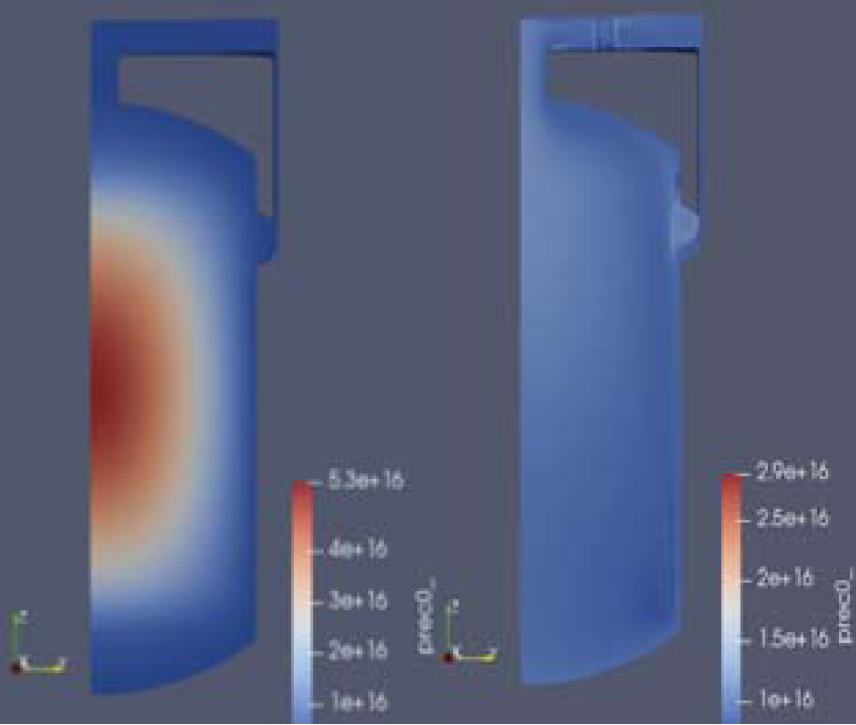
\includegraphics[scale=0.25]{images/dnp1.PNG}
  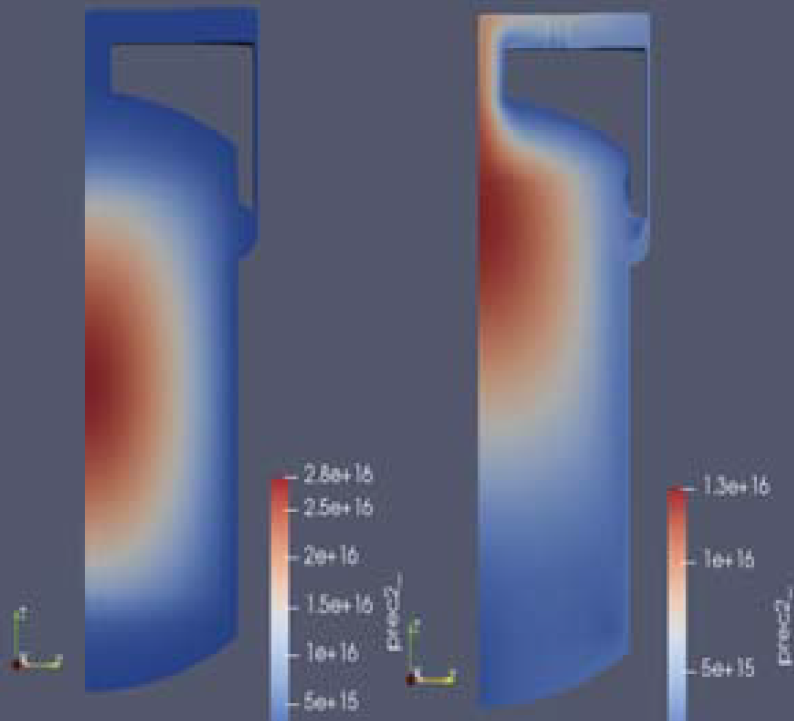
\includegraphics[scale=0.25]{images/dnp3.PNG}
  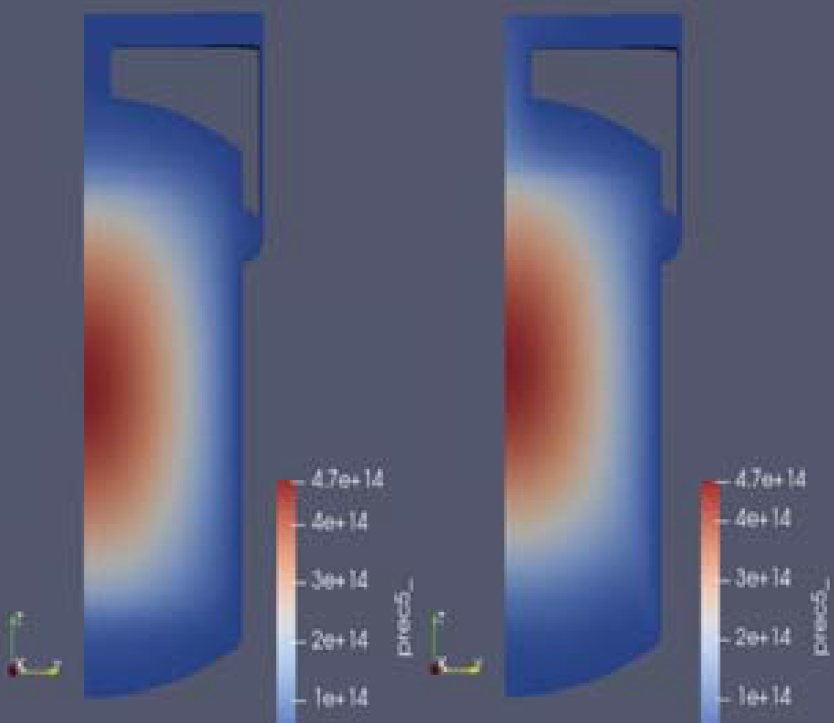
\includegraphics[scale=0.25]{images/dnp6.PNG}
  \caption{Plots of DNP concentrations in the molten salt reactor experiment \cite{shi_gen-foam_2021}. The left side of each image shows concentration with no flow, while the right shows the concentration with a 1200 gallon per minute flow rate. Top Left) Longest lived DNP group. Top Right) Third longest lived DNP group. Bottom) Shortest lived DNP group.}
   \label{fig:genfoam_dnp_locations}
\end{figure}

From these images, it can be seen that for the long shortest lived DNPs, the movement of the fuel does not have any significant impact upon the DNP distribution when compared to static fuel. This is reasonable since the precursors do not live for very long in this group, so they do not have much chance to travel. For the intermediate DNP group, there is a clear shift in the direction of the fuel flow, which causes more precursors to produce delayed neutrons in the less important piping  and upper plenum regions. The longest lived DNP group seems to be spread almost equally throughout the entire reactor, which means that those delayed neutrons are contributing significantly less to the overall neutron economy. Additionally, this reduces the overall effective delayed neutron fraction since the delayed neutrons are in less important regions. This directly affects the controllability of the reactor through the reactor period, which is heavily dependent upon the delayed neutrons.

\subsection{Depletion}

Depletion is the process of burning the fuel and simulating the changes to the materials this causes in the system. Depletion requires specific information to run properly, such as decay constants,  fission yields, and fission and transmutation cross section data. The fission and transmutation cross section data can come from a transport calculation, while the other data can be read from a data library \cite{leppanen_development_nodate}. Additionally, running depletion involves solving the Bateman equations, a generic version of which can be seen in Equation \ref{eq:Bateman_default}.

There are several different approaches to solving these equations, such as the Transmutation Trajectory Analysis (TTA) method and the Chebyshev Rational Approximation Method (CRAM). These are the two different methods used in Serpent2, and are both built into Serpent2 \cite{leppanen_serpent_2015}. Other codes may use external software to compute depletion, such as REM used by MCNP and ORIGEN-S used by KENO-VI \cite{aufiero_extended_2013}. Another code, aside from Serpent2, that contains built-in depletion solvers is ERANOS \cite{aufiero_extended_2013}.

The purpose behind solving these equations and having depletion models is to generate an accurate representation of the composition of the target materials during reactor operation. This is important in determining how long the reactor can run, how the safety of the reactor develops over time, and how operation may have to change to adjust to the new reactor state. For molten salt reactors, depletion also allows for information regarding fresh fuel feed rate and fission product removal rates, as well as how variations of those parameters can affect reactor performance and behaviour.

\subsection{The Molten Salt Breeder Reactor}

The molten salt breeder reactor (MSBR) is a useful design to analyze for several reasons. Because it is a molten salt reactor, online reprocessing is used within the design. In addition, it contains an inner and outer zone, each of which has different neutronic behaviour \cite{robertson_conceptual_1971}. More specifically, the inner zone has a softer spectrum, a higher fission rate, and a 13\% fuel-to-graphite ratio \cite{park_whole_2015}. The outer zone has a harder spectrum, a higher breeding rate, and a 37\% fuel-to-graphite ratio. The inner and outer zones prove to be an issue when accurately modeling using a unit-cell or one-region approach, as those models are unable to capture the different characteristics of each region \cite{rykhlevskii_modeling_2019}. The differences in the regions can also be seen in Figure \ref{fig:msbr_ryklev}, which allows for the difference in the fuel-to-graphite ratio to be visually noticeable.

\begin{figure}[H]
  \centering
  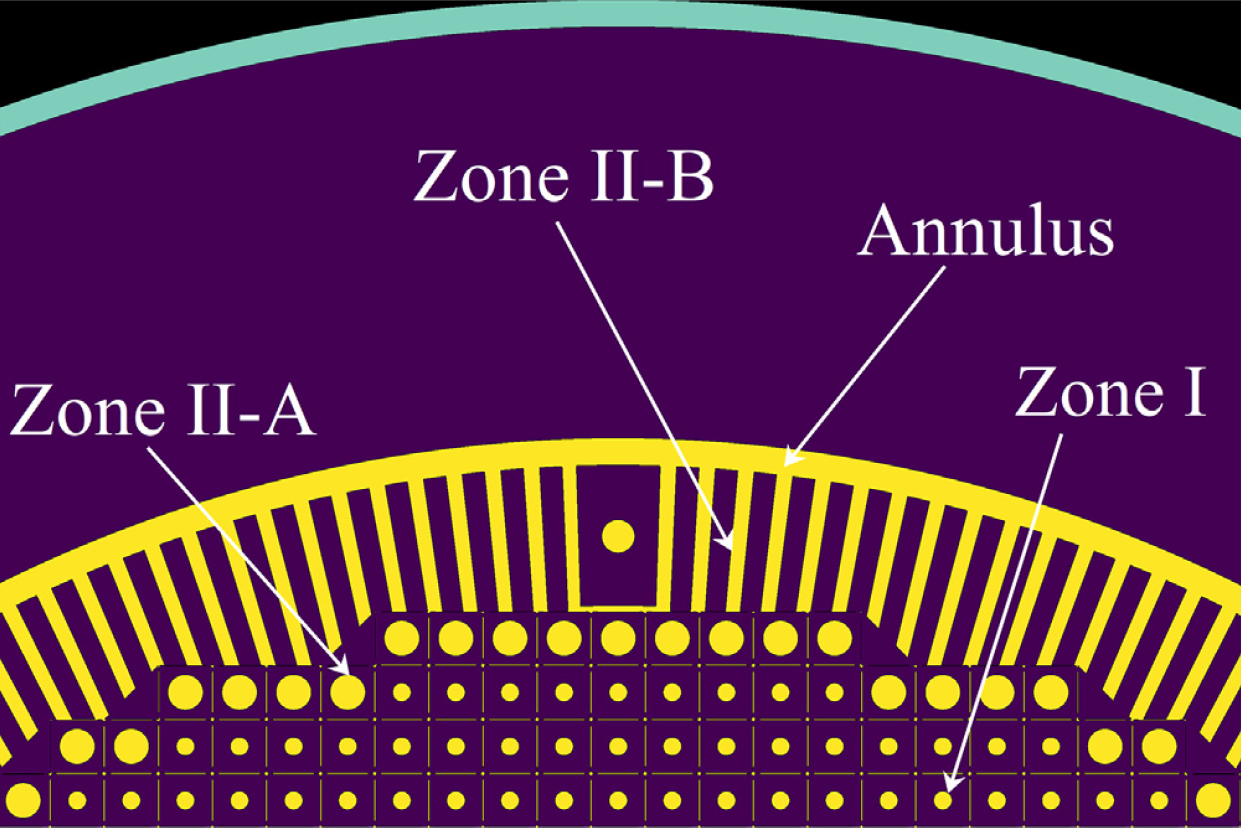
\includegraphics[scale=0.25]{images/msbr_ryk_1.PNG}
  \caption{MSBR core axial slice showing the different regions from \cite{rykhlevskii_modeling_2019}. Zones II-A and II-B are where the spectrum is harder and there is increased breeding. Zone I is where there is more fission and a softer spectrum. The yellow is fuel salt, the purple is graphite, and the cyan is the reactor vessel.}
   \label{fig:msbr_ryklev}
\end{figure}

For the online reprocessing aspect of the reactor, there are several mechanisms that contribute, as can be seen in Figure \ref{fig:msbr_robertson}. This figure shows how the reactor (1) links with the fuel salt pump (3), entrainment separator (14), and gas separator (13). The elements which are to be extracted, as well as their cycle times, are shown in Table \ref{tab:msbr_cycle_times}.


\begin{figure}[H]
  \centering
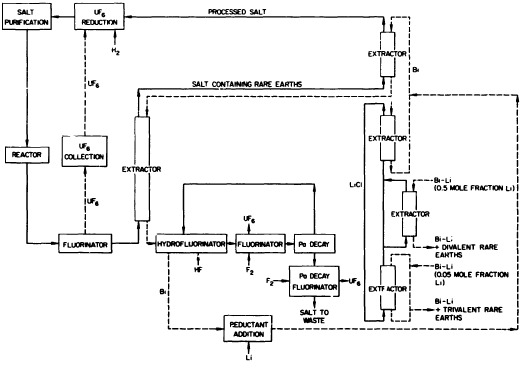
\includegraphics[scale=0.45]{images/msbr_flows_robertson.PNG}
  \caption{MSBR simplified flow diagram from \cite{robertson_conceptual_1971} showing part of primary side.}
   \label{fig:msbr_robertson}
\end{figure}

\begin{table}[H]
\renewcommand{\arraystretch}{1.25}
\caption{MSBR Online Reprocessing Cycle Times \cite{robertson_conceptual_1971}}
\label{tab:msbr_cycle_times}
\begin{center}
\begin{tabular}{ | p{0.27\linewidth} | p{0.25\linewidth} | p{0.35\linewidth} |}
 \hline
 Reprocessing Group & Element(s) & Cycle Time (Full Power)\\
 \hline
 \hline
 Rare Earths & Y, La, Ce, Pr, Nd, Pm, Sm, Gd & 50 days\\
 Rare Earths & Eu & 500 days\\
 Noble Metals  & Se, Nb, Mo, Tc, Ru, Rh, Pd, Ag, Sb, Te & 20 seconds\\
 Seminoble Metals & Zr, Cd, In, Sn &  200 days\\
 Gases & Kr, Xe & 20 seconds\\
 Volatile Fluorides & Br, I & 60 days\\
 Discard & Rb, Sr, Cs, Ba & 3435 days\\
 Protactinium & Pa (233) & 3 days\\
 Higher Nuclides & Np (237), Pu (242) & 16 years\\
 \hline
\end{tabular}
\end{center}
\end{table}

From SaltProc's MSBR example, the removal of each group can be attributed to a particular process within the physical system \cite{rykhlevskii_modeling_2019}. The entrainment separator is used to remove the gases; a nickel mesh is used to remove noble metals, seminoble metals, and volatile fluorides; and various processes given by Robertson are lumped together into the liquid metal process which removes rare earths, discard, and protactinium. The higher nuclides are removed at such an infrequent rate that they are not included within the SaltProc processes. The MSBR design removes the protactinium with the intent that the protactinium-233 will not absorb neutrons and will instead be fed out of the core to decay into uranium-233, which can then be fed back into the core.


\subsection{MSR Modeling Approaches}

*Temporarily split into different subsubsections. Perhaps generate a large table for the different approaches used, whether they use a full 3d core model, continuous/batch, how long they ran for, etc.*

\begin{table}[H]
\renewcommand{\arraystretch}{1.25}
\caption{Molten Salt Reactor Models}
\label{tab:codes_types}
\begin{center}
\begin{tabular}{ | c | c | c | c | c | c | c | }
 \hline
 Code(s) & Reprocessing & Model & Reactor & Scale & Step & Ref.\\
 \hline
 \hline
 Serpent2 & Batchwise & Full 3D & MSBR & 60 Years & 3 Days & \cite{rykhlevskii_modeling_2019}\\
 \hline
\end{tabular}
\end{center}
\end{table}


\subsubsection{SaltProc}

\cite{rykhlevskii_modeling_2019}

\subsubsection{Serpent2}
%http://montecarlo.vtt.fi/

\cite{aufiero_extended_2013} continuous

\cite{auero_modication_nodate} continuous

\subsubsection{MCNP}

\cite{park_whole_2015} batch (MSBR)

\cite{aufiero_extended_2013}

\subsubsection{SCALE}

ChemTriton \cite{betzler_molten_2017} \cite{jr_vicente_valdez_modeling_2020}

\subsubsection{ERANOS}

Uses continuous removal of non-soluble fission products, batch removal of soluble fission products\cite{fiorina_preliminary_2012}

\cite{aufiero_extended_2013}

\subsubsection{KENO-VI}

\cite{aufiero_extended_2013}

\subsubsection{Moltres}

\subsubsection{Computational Fluid Dynamics}

GenFOAM \cite{shi_gen-foam_2021}

% Gen-foam, Open-foam, anything else.

